\documentclass{crypto-exercise}
\usepackage{amsthm}
\usepackage{tikz}
\author{Sven Laur}
\contributor{}
\editor{}
\tags{false positives, false negatives, statistical distance}


\begin{document}
\begin{exercise}{Maximal region of feasible distinguishers}
For any distinguisher $\AD$ and two distributions $\XXX_0$ and $\XXX_1$, define the false-positive rate
\begin{align*}
\alpha(\AD)=\pr{x\gets\XXX_0: \AD(x)=1}\enspace\phantom{.}
\end{align*}
and the false‑negative rate as
\begin{align*}
\beta(\AD)=\pr{x\gets\XXX_1: \AD(x)=0}\enspace.
\end{align*}
Then it is straightforward to prove the following inequality 
\begin{align}\label{ineq}
1-\SD_x(\XXX_0,\XXX_1)\leq \alpha(\AD) +\beta(\AD)\leq 1+\SD_x(\XXX_0,\XXX_1)
\end{align}
Define distributions $\mathcal{X}_0$ and $\mathcal{X}_1$ over the set $\{0,1,2\}$ such that $\SD_x(\XXX_0,\XXX_1)=\tfrac{1}{2}$, and such that every point in the feasible region~\eqref{ineq} has a corresponding distinguisher. In particular construct distinguishers $\mathcal{A}_1, \mathcal{A}_2,\ldots, \mathcal{A}_6$ as indicated in the following figure. 
\begin{center}
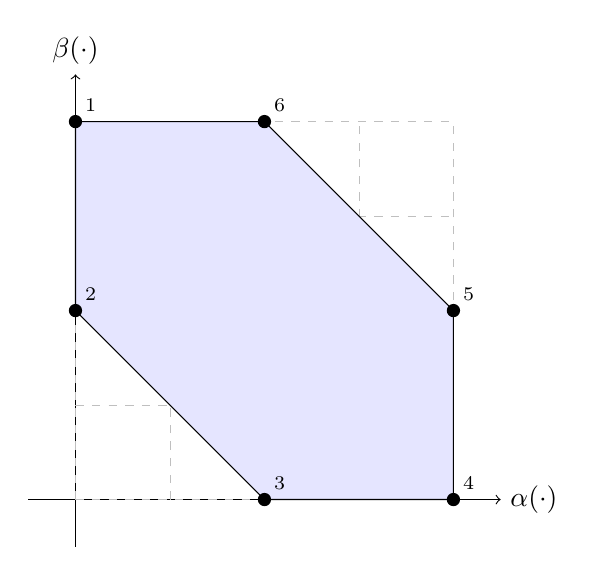
\begin{tikzpicture}[scale=1.2]
    % Axes
    \draw[->] (-0.5,0) -- (4.5,0) node[right] {$\alpha(\cdot)$};
    \draw[->] (0,-0.5) -- (0,4.5) node[above] {$\beta(\cdot)$};

    % Grid (optional)
    \draw[help lines, dashed, gray!50] (0,0) grid (4,4);

    \fill[fill=blue!10, draw=black] (0,4) -- (0,2) -- (2,0) -- (4,0) -- (4,2) --(2,4) -- cycle;

    % Points
    \fill (0,4) circle (2pt) node[anchor=south west] {$\AD_1$};
    \fill (0,2) circle (2pt) node[anchor=south west] {$\AD_2$};
    \fill (2,0) circle (2pt) node[anchor=south west] {$\AD_3$};
    \fill (4,0) circle (2pt) node[anchor=south west] {$\AD_4$};
    \fill (4,2) circle (2pt) node[anchor=south west] {$\AD_5$};
    \fill (2,4) circle (2pt) node[anchor=south west] {$\AD_6$};

\end{tikzpicture}
\end{center}



\end{exercise}


\begin{solution}
\end{solution}

\end{document}

